%%%%%%%%%%%%%%%%%%%%%%%%%%%%%%%%%%%%%%%%%%%%%%%%%%%%%%%%%%%%%%%%%%
\section{Smart Grids}
\label{sec:smartgrids}


En las últimas décadas, se ha observado una transformación integral del modelo asociado a la red eléctrica convencional. El aumento de la energía demandada por los usuarios finales y los requisitos cada vez mayores de la industria ha tenido como consecuencia que algunos países hayan intentado diseñar redes eléctricas agrupadas en un conjunto de grandes redes nacionales. De este modo, todas las fuentes energéticas disponibles pueden estar conectadas para ser gestionadas conjuntamente en función de la demanda recibida, además de conseguir una coordinación a alto nivel. \cite{smartgrid_overview}

\vspace{3mm}

Sin embargo, una red eléctrica no se puede definir como una entidad única e independiente, pues se trata de una agregación de redes, compañías energéticas y operadores que trabajan en distintos niveles de comunicación. Es por ello que la idea de desarrollar una gran red nacional encuentra cierto equilibrio energético, pero no llega a los altos porcentajes de eficiencia que pueden proveer las redes inteligentes energéticas o de otra forma, las \acrfull{sgs}. 

\vspace{3mm}

La iniciativa sobre redes inteligentes del \gls{ieee}, califica a las \textit{smart grids} \cite{ieee} como ``imperativas y revolucionarias que implican nuevas capacidades de comunicación y control, fuentes de energía, modelos de generación y adherencia a estructuras regulatorias transjurisdiccionales''. Por otro lado, en el año 2009, el Departamento de Energía de Estados Unidos \cite{us} determinó en su reporte anual sobre \gls{sg}s los siguientes objetivos principales que se perseguían con el desarrollo de este tipo de redes: 

\begin{itemize}
  \item Permitir una participación activa de los clientes en el sistema.
  \item Integrar todas las opciones de generación y almacenamiento de energía.
  \item Ofertar nuevos productos y servicios.
  \item Proporcionar energía de calidad y satisfacer un gran rango de necesidades.
  \item Optimizar el uso de los recursos y aumentar la eficiencia.
  \item Dar una respuesta rápida ante emergencias y problemas producidos en la red.
\end{itemize}

\vspace{1mm}

Tomando en consideración estos objetivos, se puede definir una \gls{sg} como una red inteligente con la capacidad de distribuir los suministros de energía de forma optimizada a los usuarios, basándose en la información que recoge de los mismos. Es por ello que supone una actualización digital de las redes de distribución y transmisión a larga distancia para incorporar sistemas de monitorización y control a tiempo real (ver Figura \ref{fig:bidireccional2}). \cite{iotfutura} 

\vspace{3mm}

\begin{figure}[H]
  \centering
  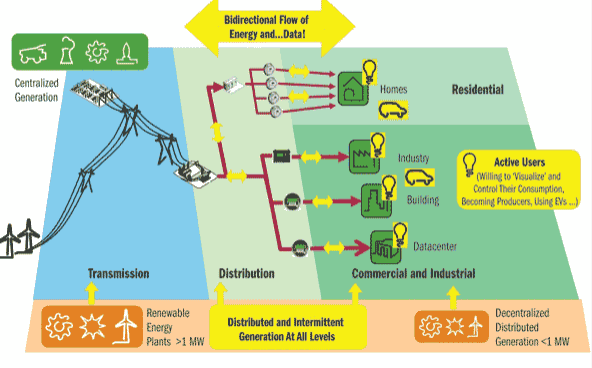
\includegraphics[width=0.9\textwidth]{img/teoria/sg.png}
  \caption{Red de distribución y flujo bidireccional de datos y energía en una \textit{smart grid} \cite{sins}}
  \label{fig:bidireccional}
\end{figure}

\vspace{3mm}

Su base se asienta en el diseño de sistemas inteligentes coordinados capaces de obtener tanto la información respectiva a la demanda o requisitos energéticos de cada zona como la de la disponibilidad de recursos a partir de las diferentes fuentes de producción existentes. Todo ello conduce al desarrollo de un plan estratégico de distribución energética para poder conectar a todas las entidades participantes en la red entre sí. 

\vspace{3mm}

Además, en cuanto al factor medioambiental, las \gls{sg}s son un concepto clave en la transición energética y en el proceso de descarbonización. La aplicación de una distribución energética inteligente y la posibilidad de integrar al sistema fuentes renovables y limpias potencian el desarrollo de ciudades sostenibles y permiten una gran reducción de emisiones de CO2. \cite{repsol} \cite{iberdrola}


%%%%%%%%%%%%%%%%%%%%%%%%%%%%%%%%%%%%%%%%%%%%%%%%%%%%%%%%%%%%%%%%%%
\subsection{Flujo energético y comunicación bidireccional}

Cabe destacar que una de las principales características diferenciadoras de las \gls{sg}s respecto a las redes energéticas convencionales es que se fundamentan en una comunicación bidireccional. Este factor determinante se puede apreciar en la Figura \ref{fig:bidireccional} y se traduce en una producción y una distribución dinámica y personalizada hacia cada uno de los usuarios de la red. 

\vspace{3mm}

Es decir, en una red tradicional al ser unidireccional, se provee energía desde el distribuidor hacia el consumidor sin llevar a cabo ningún análisis estadístico sobre el consumo que se está produciendo en las líneas finales en un determinado instante temporal. En cambio, en el contexto de las \gls{sg}s, se pone el foco en las acciones de los usuarios y en la consecuente asignación de patrones de consumo eléctrico que permita predecir el comportamiento futuro de los mismos. Sin embargo, como se expondrá más adelante en la Sección \ref{sec:consumo}, este proceso de clasificación de usuarios requerirá del análisis de grandes volúmenes de datos adquiridos a tiempo real, por lo que se aumentará la complejidad del sistema a costa de alcanzar la eficiencia. \cite{conventional}

\vspace{3mm}

Bajo la premisa de la característica de red bidireccional, se puede expresar que los propios usuarios son el gran pilar sobre el que se cimienta el sistema. En comparación a la red eléctrica tradicional, toman un papel mucho más activo monitorizando continuamente su comportamiento eléctrico y recopilando información para trasladarla al resto de la red. Esto tiene como ventaja una gran reducción de los costes derivados de la distribución y transmisión en el sistema, ya que se evita proporcionar más cantidad de energía de la requerida por las líneas finales. \cite{iotfutura}

\vspace{3mm}
\pagebreak

Es por ello que se emplea una Infraestructura Avanzada de Medición (del inglés \gls{ami}) con una interfaz constituida por varias capas o niveles como se puede apreciar en la Figura \ref{fig:bidireccional2}. De esta forma, se dividen los flujos de comunicación entre las diferentes entidades que componen la red para permitir una mejor gestión de los mismos. \cite{us}

\vspace{3mm}

\begin{figure}[H]
  \centering
  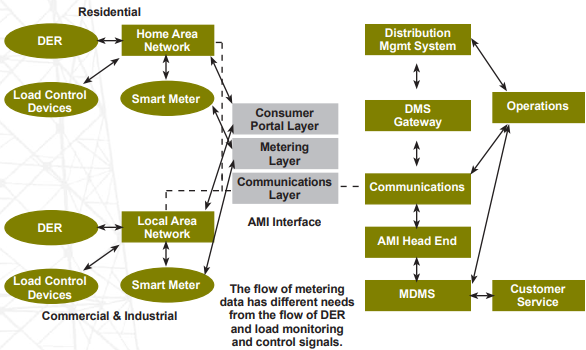
\includegraphics[width=0.9\textwidth]{img/teoria/bidir.png}
  \caption{Infraestructura de una interfaz \acrshort{ami} para el flujo bidireccional de energía y datos \cite{us}}
  \label{fig:bidireccional2}
\end{figure}


%%%%%%%%%%%%%%%%%%%%%%%%%%%%%%%%%%%%%%%%%%%%%%%%%%%%%%%%%%%%%%%%%%
\subsection{Prosumidores y microgrids}
\label{sec:prosu}

Dentro del presente contexto, en referencia a los usuarios, es preciso introducir el término de prosumidor \cite{transactive}. Se puede determinar como prosumidora a toda entidad o usuario final que tiene la capacidad de producir de forma alternativa recursos energéticos, además de poder consumirlos. En la Figura \ref{fig:prosumer}, se puede visualizar cómo se estructura la \gls{sg} en un conjunto de distintas comunidades o agregaciones de prosumidores con el fin de crear microrredes de distribución y almacenamiento energético (del inglés \textit{microgrids}).

\vspace{3mm}

En este caso es imprescindible que los equipos y dispositivos dedicados a la generación de electricidad se encuentren dentro de la microrred o en una ubicación cercana a la misma. Así, se podrá abastecer a los usuarios del conjunto de forma eficiente, reduciendo los costes relacionados con la transmisión energética. Este tipo de esquema puede ser aplicado en diferentes entornos, como pueden ser los residenciales, industriales o agrícolas, para conseguir descentralizar la gestión de los recursos. 

\vspace{3mm}
\pagebreak

Sin embargo, debe existir cierta gestión externa y coordinada de todas estas microrredes o comunidades de usuarios. Esta es llevada a cabo por una entidad denominada como operador del sistema distribuido (del ingles \gls{dso}) \cite{transactive} \cite{dso}. Algunas de sus funciones principales se basan en asegurar el abastecimiento de recursos en el interior de las microrredes en función de la demanda existente y en supervisar el estado operativo la infraestructura de red para garantizar su estabilidad y seguridad. 

\vspace{3mm}

\begin{figure}[h!]
  \centering
  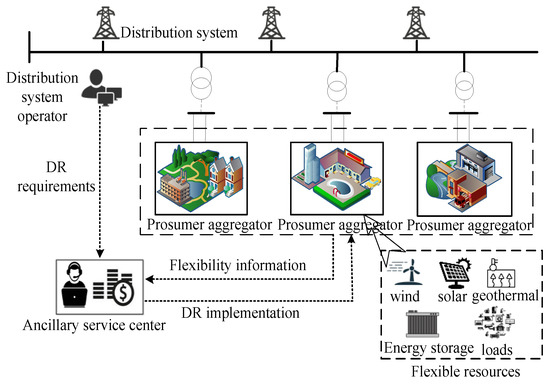
\includegraphics[width=0.8\textwidth]{img/teoria/prosumer.jpg}
  \caption{Estructura de la respuesta a la demanda en el contexto de una \acrshort{sg} con prosumidores \cite{transactive}}
  \label{fig:prosumer}
\end{figure}

\vspace{3mm}

Por otro lado, se encuentra también la figura del centro de servicios auxiliares \cite{transactive}, que se encarga de recibir la información sobre los recursos energéticos de los prosumidores y cuantificar en función de la oferta y demanda el beneficio económico que obtendrán los prosumidores. Estos normalmente son gestionados por los operadores del mercado eléctrico, pero puede variar según la región o el país.

\vspace{3mm}

\subsubsection{Mercado energético}

En la Figura \ref{fig:market} se ilustra la estructura del modelo que presenta el mercado energético. Por un lado, las agregaciones de prosumidores posibilitan el autoconsumo y la compartición de los recursos generados por sí mismos con los demás participantes de la microrred, además de con el resto de la \gls{sg}. La mayoría de los prosumidores, sobre todo en entornos residenciales son de menor tamaño y tienen mayores complicaciones para participar en los mercados eléctricos por sí mismos. 

\vspace{3mm}

\begin{figure}[h!]
  \centering
  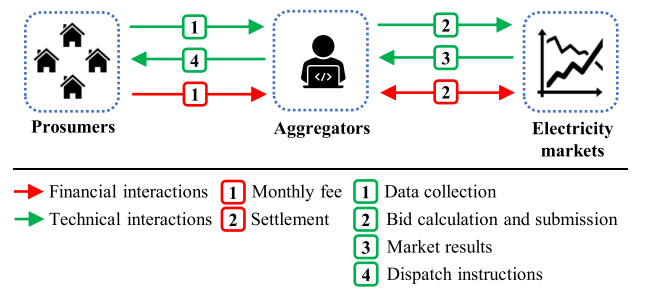
\includegraphics[width=0.8\textwidth]{img/teoria/market.png}
  \caption{Modelo basado en las interacciones de los agregadores con los prosumidores y el mercado eléctrico \cite{business}}
  \label{fig:market}
\end{figure}

Por ello, los agregadores \cite{bidding} \cite{transactive} se encargan de facilitar esta tarea para que una cantidad de prosumidores locales puedan actuar en conjunto como fijadores de precios de compra/venta en el mercado eléctrico global. Es decir, cada agregador se encarga de representar a un conjunto determinado de prosumidores y opera como entidad intermediaria entre los mismos y el conjunto de mercados energéticos. Cada prosumidor debe pagar a cambio un plan mensual a la compañía para cubrir los costes eléctricos y así, dejar la responsabilidad de las transacciones a los agregadores para que operen de forma flexible.

\vspace{3mm}

Por otro lado, en esta operativa también incide el \gls{dso}, el cual se encarga de que las transacciones de compra/venta sigan el cumplimiento de los estándares y regulaciones establecidos en el mercado energético. A partir del funcionamiento expuesto y de la Figura \ref{fig:market}, se pueden diferenciar los tipos de interacciones que se producen en este modelo \cite{business}:

\vspace{3mm}

\begin{itemize}
  \item Interacciones técnicas 
    \begin{enumerate}
      \item Recopilación y adquisición de datos sobre los recursos de los prosumidores para su posterior procesamiento en los agregadores.  
      \item Cuantificación y presentación de ofertas desde los agregadores hacia los mercados mayoristas de electricidad.
      \item Comunicación de los resultados de diferentes mercados a los agregadores.
      \item Envío de instrucciones o recursos distribuidos en función de los resultados del mercado.      
    \end{enumerate}

  \item Interacciones financieras
  \begin{enumerate}
    \item Pago de tarifa mensual de cada prosumidor al agregador.
    \item Liquidación de las transacciones trasladadas desde los prosumidores en el mercado eléctrico (cobro por demanda y pago por generación).    
  \end{enumerate}
\end{itemize}

\vspace{1mm}

En cuanto al proceso de fijación de precios, generalmente, se adoptan tarifas minoristas dinámicas según el instante temporal, como pueden ser la fijación de precios por tiempo de uso (del inglés \gls{tou}) o en tiempo real (del inglés \gls{rtp}). Dentro de este contexto es preciso introducir los programas de gestión del lado de la demanda (del inglés \gls{dsm}). 

\vspace{3mm}

Como término, un programa \gls{dsm} es un programa basado en el control de las interacciones de consumo y de gestión de cargas residenciales desde el lado del cliente. Considerando este modelo de interacciones, se puede expresar que un \gls{dsm} tiene como pilar fundamental la distribución de recursos energéticos de manera eficiente y acorde a la demanda y a la oferta. Permite reducir el coste de la adquisición energética y los costes asociados a la distribución como consecuencia de minimizar el número de interacciones necesarias entre el prosumidor y el resto de entidades del sistema. \cite{dsm}

\vspace{3mm}

Por lo tanto, volviendo a los modos de dinamización de las tarifas, si por ejemplo se emplea \gls{rtp}, se buscará lograr el equilibrio de la demanda en tiempo real, modificando las cargas de los consumidores en las horas pico \cite{rtp}. Es decir, cada uno de los usuarios actuará individualmente en función de los precios dinámicos en el tiempo, comunicándose directamente con la compañía energética como se muestra en la Figura \ref{fig:dsm1}. 

\vspace{3mm}

\begin{figure}[h!]
  \centering
  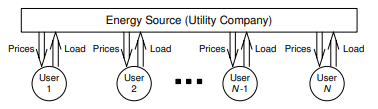
\includegraphics[width=0.75\textwidth]{img/teoria/dsm1.png}
  \caption{Estrategia de \acrshort{dsm} basada en interacciones individuales de cada consumidor con la compañía \cite{pricing}}
  \label{fig:dsm1}
\end{figure}

\vspace{3mm}

Con este proceso, como el consumidor puede saber en tiempo real la tarifa a la que está consumiendo energía, puede trasladar su propia carga desde las horas donde el precio es más alto (horas pico) a las de precio menor (horas valle). Esta gestión produce por tanto, menores picos de demanda y contribuye a la bajada de los precios. \cite{dsm} \cite{pricing}

\vspace{3mm}

No obstante, el diseño de un programa \gls{dsm} ideal en el contexto de las \gls{sg}s debería permitir también las interacciones entre los mismos prosumidores dentro de una zona residencial o microgrid. Estas interacciones generalmente se automatizan a través de equipos dedicados a una comunicación digital bidireccional. Como se aprecia en la Figura \ref{fig:dsm2}, este proceso tiene como fin conducir a una coordinación de las acciones respectivas a las cargas de un área determinada. Por tanto, en este caso la monitorización de las cargas totales para todos los nodos participantes en un instante determinado aportará la información necesaria sobre la relación entre la potencia pico y promedio (del inglés \gls{par}) y contribuirá a la fijación del precio unitario para ese mismo instante. \cite{pricing}

\vspace{3mm}

\begin{figure}[h!]
  \centering
  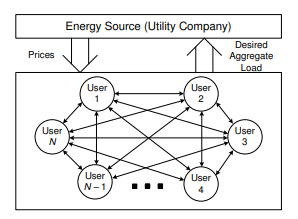
\includegraphics[width=0.65\textwidth]{img/teoria/dsm2.png}
  \caption{Estrategia de \acrshort{dsm} para \acrshort{sg}s basada en interacciones entre los usuarios y la compañía \cite{pricing}}
  \label{fig:dsm2}
\end{figure}


%%%%%%%%%%%%%%%%%%%%%%%%%%%%%%%%%%%%%%%%%%%%%%%%%%%%%%%%%%%%%%%%%%
\subsection{Estructura de una Smart Grid}

Una \gls{sg} está constituida por múltiples elementos diferentes como se puede visualizar en la Figura \ref{fig:estructura_sg}. Cada uno de ellos está dedicado a uno de los procesos principales, que se pueden dividir en generación, distribución y consumo. \cite{smartgrid_overview}

\begin{figure}[h!]
  \centering
  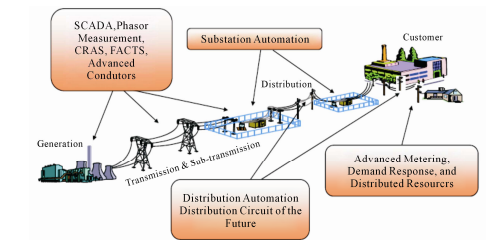
\includegraphics[width=1\textwidth]{img/teoria/estructura_sg.png}
  \caption{Estructura de componentes de una \acrshort{sg} \cite{smartgrid_overview}}
  \label{fig:estructura_sg}
\end{figure}

\subsubsection{Generación}

Como ya se introducía en la Sección \ref{sec:prosu}, dentro de una \gls{sg}, el prosumidor se trata de la figura que potencia principalmente el uso de energías renovables, las cuales pueden ser obtenidas por ejemplo a partir de generadores térmicos fotovoltaicos (del inglés \gls{pvt}) o de turbinas eólicas. Para posibilitar posteriormente el uso de la energía generada, esta debe ser convertida y acondicionada mediante dispositivos dedicados, como pueden ser las unidades combinadas de calor (del inglés \gls{chp}) o las de conversión a gas (del inglés \gls{p2g}). \cite{transactive}

\vspace{3mm}

Las unidades \gls{chp} \cite{chp}, como se puede apreciar en la Figura \ref{fig:chp}, llevan a cabo un aprovechamiento del calor residual que deriva del proceso de generación de electricidad. Se emplean como respaldo eléctrico, ya que se componen de sistemas de almacenamiento de energía térmica (del inglés \gls{tes}) para poder separar la producción y el uso del calor y la energía. Luego, este calor almacenado se puede emplear en aplicaciones térmicas como la calefacción o en otros procesos enfocados a entornos industriales. \cite{chp2}

\vspace{3mm}

\begin{figure}[h!]
  \centering
  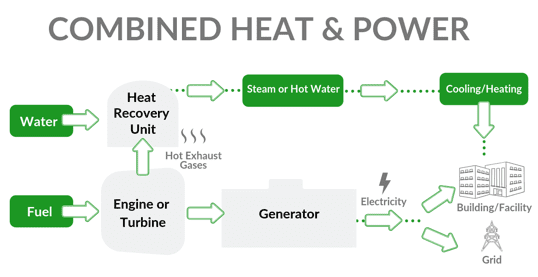
\includegraphics[width=0.95\textwidth]{img/teoria/chp.png}
  \caption{Esquema de funcionamiento de una unidad \acrshort{chp} \cite{chp}}
  \label{fig:chp}
\end{figure}

\vspace{3mm}

Es por ello que las unidades \gls{chp} mejoran la eficiencia del sistema energético, contribuyendo a un uso mucho más eficaz de los recursos y a una reducción de las pérdidas que se producen en la transmisión. Además del \gls{tes}, utilizado para almacenar el calor producido, una unidad \gls{chp} también se constituye de un motor acoplado a un generador eléctrico para llevar a cabo el proceso de generación de electricidad y calor. Como se puede apreciar en la Figura \ref{fig:chp2}, todas las operaciones de la unidad y las interacciones que se producen entre módulos se coordinan desde el gestor de operaciones para que se produzca un correcto funcionamiento.

\vspace{3mm}

\begin{figure}[h!]
  \centering
  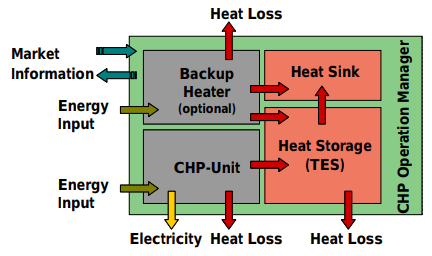
\includegraphics[width=0.65\textwidth]{img/teoria/chp2.png}
  \caption{Gestión de operaciones en una unidad \acrshort{chp} \cite{chp2}}
  \label{fig:chp2}
\end{figure}

\vspace{3mm}
\pagebreak

Por otro lado, la unidad \gls{p2g}, mencionada anteriormente, se encarga de la conversión de la electricidad en gases sintéticos, como son el hidrógeno o el metano. Es de gran importancia, ya que este tipo de gases son más fácil de transportar y almacenar que la electricidad, por lo que se simplifica la gestión energética. Como se puede apreciar en la Figura \ref{fig:p2g}, el objetivo del \gls{p2g} se basa en descomponer el agua mediante un proceso de electrólisis a partir de electricidad proveniente de fuentes renovables. Después, el hidrógeno que se produce se puede utilizar directamente o procesarlo de forma adicional en metano.~\cite{transactive} 

\vspace{3mm}

\begin{figure}[h!]
  \centering
  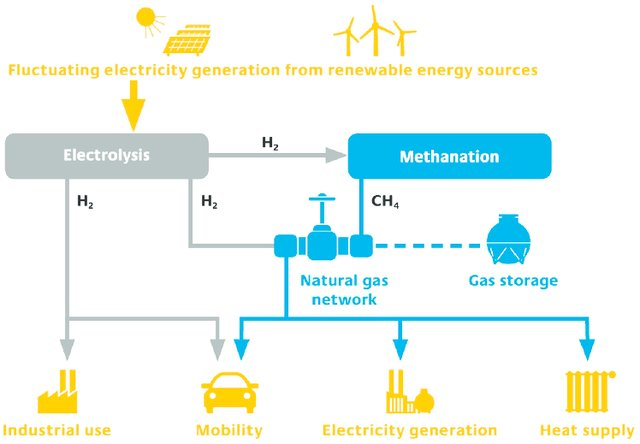
\includegraphics[width=0.85\textwidth]{img/teoria/p2g.jpg}
  \caption{Representación del proceso \acrshort{p2g} \cite{p2g}}
  \label{fig:p2g}
\end{figure}

\vspace{3mm}
\pagebreak

Dentro del contexto de la generación de energía también es importante destacar algunos equipos, como son los sistemas de control y adquisición de datos (del inglés \gls{scada}) \cite{scada}. Estos pueden ser instalados en generadores, como paneles solares fotovoltaicos o turbinas eólicas, consiguiendo una monitorización remota de los mismos. Mediante la información recopilada a tiempo real permiten conocer los niveles de generación y establecer una predicción de la disponibilidad energética que habrá en el sistema o en un área determinada del mismo.

\vspace{3mm}

\subsubsection{Distribución}

Un dispositivo importante en el campo de la distribución energética es la Unidad de Medición de Fasores (del inglés \gls{pmu}). Se emplea para medir con una alta precisión los fasores de tensión y corriente en la red eléctrica, proporcionando información relevante sobre las magnitudes y fases de las ondas sinusoidales. También, es empleado en los generadores y debe contar con una alta tasa de muestreo para capturar eventos transitorios o cambios rápidos en la red. En otros términos, debe tener la capacidad de identificar o detectar a tiempo real posibles anomalías que se puedan dar en la distribución. Teniendo esto en cuenta, se puede expresar que se trata de un componente imprescindible para comprobar y garantizar la estabilidad de la \gls{sg}. \cite{dynamic}

\vspace{3mm}

La confiabilidad y la seguridad de la red también reside en los Sistemas de Transmisión de Corriente Alterna Flexibles (del inglés \gls{facts}) \cite{facts} \cite{facts3}. Estos vienen dados por la necesidad de superar las limitaciones técnicas introducidas por las redes eléctricas, como son las térmicas o las respectivas al voltaje. En otros términos, incrementan la potencia transmitida y aportan flexibilidad al permitir modificar de forma dinámica los parámetros eléctricos ante cambios en la configuración de la red. 

\vspace{3mm}

Los \gls{facts} incluyen todos los elementos electrónicos basados en tecnología de alta potencia y que son empleados dentro de una \gls{sg} para la transferencia de energía de CA y el control de la potencia reactiva. También, realizan tareas de reducción de impedancia en las líneas de transmisión y de optimización del factor de potencia y pueden actuar tanto a nivel individual como de forma coordinada con otros controladores. Los \gls{facts} se dividen en dos generaciones: la primera emplea interruptores controlados por tiristores y la segunda tiene como base convertidores estáticos de conmutación. En la Tabla \ref{tab:facts} se visualizan las tecnologías \gls{facts} más relevantes. \cite{facts2} \cite{facts3}

\vspace{3mm}

Poniendo el enfoque en la garantía de estabilidad de una \gls{sg}, uno de los sistemas más importantes de los expuestos en la Tabla \ref{tab:facts} es el \gls{svc} \cite{facts}. En la Figura \ref{fig:svc} se puede apreciar un ejemplo de instalación de compensador, ubicado en el municipio noruego Sylling y conectado a un sistema de 420 kV.

\vspace{3mm}

\begin{figure}[h!]
  \centering
  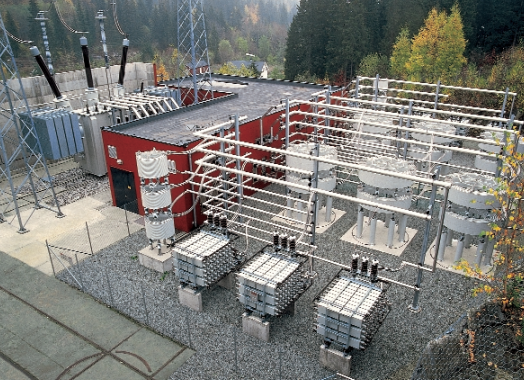
\includegraphics[width=0.8\textwidth]{img/teoria/svc.png}
  \caption{Instalación de un \acrshort{svc} en Sylling (Noruega) \cite{facts}}
  \label{fig:svc}
\end{figure}

\vspace{3mm}
\pagebreak

\begin{table}[!h]
  \centering
  \resizebox{\textwidth}{!}{
  \begin{tabular}{| c | c | m{6cm} |}
  \hline
  \rowcolor[HTML]{EFEFEF}
  Generación & Tipo & \multicolumn{1}{c|}{Descripción} \\ \hline
  \multirow{2}{*}{1º} 

  & \gls{tcsc} & Controla el flujo de potencia tanto reactiva como activa por la línea de transmisión mediante el ajuste de impedancia en serie y amortigua las oscilaciones.
  
  \\ \cline{2-3}

  & \gls{svc} & Absorbe o suministra potencia reactiva según las necesidades de una línea de transmisión a través de la variación de la susceptancia en paralelo. Ayuda a mantener el voltaje estable en la red y proveen un aumento de la capacidad de transferencia de energía.

  \\ \hline
  \multirow{4}{*}{2º} 
  
  & \gls{statcom} & Compensa la potencia reactiva al igual que el \gls{svc}, pero en este caso empleando electrónica de potencia para proporcionar una respuesta más rápida.

  \\ \cline{2-3} 

  & \gls{upfc} & Combina las funciones de un \gls{tcsc} y un \gls{svc}, teniendo la capacidad de controlar en una línea de transmisión tanto la impedancia en serie como la susceptancia en paralelo.

  \\ \cline{2-3} 

  & \gls{sssc} & Modifica dinámicamente la impedancia y es capaz de controlar la fase y la amplitud de la tensión en la línea.

  \\ \cline{2-3} 

  & \gls{ipfc} & Conecta varias líneas de transmisión en paralelo. No obstante, modula la impedancia y la fase de la tensión de cada línea de transmisión de forma independiente, lo que permite operar sobre el flujo de potencia de una forma controlada. Mejora la capacidad de transmisión y reduce las pérdidas energéticas. 
  
  \\ \hline
  \end{tabular}
  }
  \caption{Tecnologías FACTS de 1ª y 2ª generación}
  \label{tab:facts}
\end{table}

\pagebreak

\vspace{3mm}

Los compensadores estáticos son capaces de detectar grandes caídas de tensión resultantes a la producción de un cortocircuito o a la pérdida de líneas de transisión en un área de la red. Esto es importante, ya que una detección rápida de una avería permite restaurar en un corto período de tiempo la tensión del área afectada sin que el problema escale a otras partes de la red. En otros términos, aísla este área del resto de la red eléctrica. Además, el \gls{svc} asegura que el proceso de restauración se produzca paulatinamente para que los efectos producidos por el cortocircuito sean prácticamente imperceptibles en los puntos de carga del área afectada. 

\vspace{3mm}

Siguiendo en el ámbito de la distribución energética, es importante también exponer las tecnologías enfocadas a la transmisión de electricidad a larga distancia, como son las Corriente Continua de Alto Voltaje (del ingles \gls{hvdc})~\cite{hvdc}. Como su nombre indica, utilizan corriente continua para ello, lo que minimiza las pérdidas en el proceso de transmisión respecto al caso de la Corriente Alterna de Alto Voltaje (del ingles \gls{hvac}), además de permitir portar mucha más potencia. Esto es fundamental cuando se pretende integrar al sistema global fuentes de energía ubicadas en áreas remotas, sobre todo dentro del contexto de las \gls{sg}s. Generalmente, las fuentes de energías renovables, como pueden ser la solar o la eólica, se encuentran alejadas de los puntos geográficos con mayor demanda y se requiere una respuesta rápida ante cambios de carga para mantener la estabilidad del sistema. 

\vspace{3mm}

Entrando en detalle, cuando se transmiten grandes cantidades de potencia a largas distancias con líneas de \gls{hvac}, se generan ángulos eléctricos entre los voltajes y las corrientes en la línea muy grandes que pueden producir oscilaciones descontroladas y por tanto, desencadenar inestabilidades que llegarían a escalar a lo largo del sistema. Las tecnologías \gls{hvdc} simplifican la interconexión entre microrredes y permiten una mayor integración de sistemas dedicados al almacenamiento energético para facilitar la gestión de los recursos disponibles. Sin embargo, presentan ciertas desventajas, destacando el alto coste que supone su implementación, ya que al final únicamente se pueden emplear en el caso de aplicaciones punto a punto.

\vspace{3mm}

En la Figura \ref{fig:hvdc} se muestra como ejemplo una infraestructura de transmisión de energía eólica a larga distancia. Esta energía proviene de una fuente remota y se transporta a través del medio marino para llegar hasta los usuarios. Como se puede apreciar, es necesario implementar estaciones de conversión de alto voltaje de corriente alterna a continua y viceversa en los extremos de las líneas \gls{hvdc}.

\begin{figure}[h!]
  \centering
  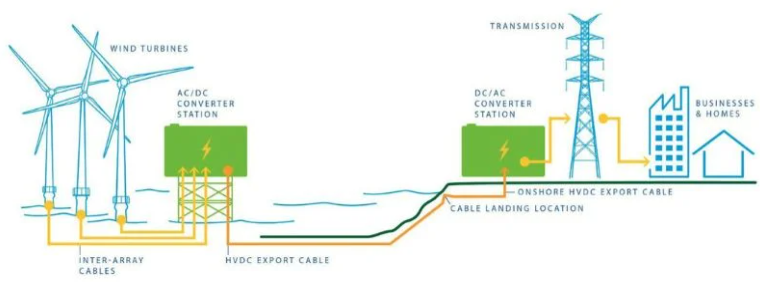
\includegraphics[width=1\textwidth]{img/teoria/hvdc.png}
  \caption{Representación de un sistema de transmisión de energía eólica con líneas \acrshort{hvdc}~\cite{hvdc2}}
  \label{fig:hvdc}
\end{figure}

\subsubsection{Consumo}
\label{sec:consumo}

Entrando en detalle en las ubicaciones finales del sistema y por tanto, en el proceso de consumo, es imprescindible conocer la cantidad de energía demandada por los clientes que pertenecen a una \gls{sg}. La instalación de sensores o medidores inteligentes (del ingles \textit{smart meters}) en las viviendas posibilitan el registro constante de datos respectivos al consumo de energía, niveles de voltaje, corriente y factor de potencia. Estos son almacenados, analizados y procesados por las distribuidoras de energía para obtener a partir de los mismos la información necesaria sobre el comportamiento de los usuarios. \cite{stab}

\vspace{3mm}

Como se había introducido en el Apartado \ref{sec:smartgrids} el proceso de adquisición de datos por parte de los usuarios se trata de uno de los pilares más relevantes de cara a la optimización energética del sistema. Los objetivos principales que se pretenden con este proceso se engloban en la reducción del consumo y la optimización de la distribución y el beneficio. Respecto a este último, las compañías energéticas a partir de su base de clientes estudian las estrategias de categorización de los mismos para definir el sistema de fijación de precios dinámicos. \cite{stab}

\vspace{3mm}

No obstante, la gestión de los sensores finales en las \gls{sg}s se caracteriza por su alta complejidad, debido a los grandes volúmenes de datos a manejar. Se requiere un procesamiento eficiente a tiempo real para analizar datos capturados de múltiples fuentes con el fin de evitar latencias o bloqueos en el sistema. Es por ello que se dificulta el empleo de herramientas convencionales de gestión de bases de datos y se requiere una solución más avanzada mediante la aplicación de tecnologías enfocadas al \textit{Big Data}. Se profundizará más sobre ello en la Sección \ref{sec:bigdata}.


%%%%%%%%%%%%%%%%%%%%%%%%%%%%%%%%%%%%%%%%%%%%%%%%%%%%%%%%%%%%%%%%%%
\subsection{Seguridad en Smart grids}
\label{sec:seg}
 
Como se ha introducido en la Sección referente a la figura del prosumidor (ver Sección \ref{sec:prosu}), el \gls{dso} tiene la capacidad de operar ante problemas y fallos en la red tomando decisiones y dando una respuesta rápida. En determinados casos, las incidencias se pueden dar por la configuración del propio sistema, si esta no se realiza de forma correcta y eficiente. No obstante, también es preciso contemplar la posibilidad de ataques externos que atenten contra el sistema de la \gls{sg}.

\vspace{3mm}

Uno de los ataques más peligrosos en este ámbito es el de Inyección de Datos Falsos (del inglés \gls{fdi}) \cite{baddata} y, como su nombre indica, se basa en la inyección de paquetes maliciosos en la red con el fin de bloquear los servicios de la misma y conseguir la autorización para realizar operaciones restringidas. El proceso se puede realizar actuando directamente a través de los sensores finales (\textit{smart meters}) o secuestrando el canal de comunicación. Algunas técnicas empleadas por los atacantes son las siguientes \cite{baddata}:

\begin{itemize}
  \item Fallo del dispositivo: Se aplica un ataque de Denegación de Servicio (del inglés \gls{dos}) a los sensores. Cabe destacar que generalmente los sensores que se encuentran en las ubicaciones finales tienen una capacidad limitada de conexión, que derivaría en grandes latencias en la comunicación de datos con el resto de entidades de la red. En este momento, el atacante se encarga de suplantar al host en cuestión para enviar los paquetes falsos en su nombre.
  \item \textit{Cracking}: Se descifran las contraseñas para obtener acceso a los equipos mediante ingeniería social o fuerza bruta. De la misma forma que el anterior, la limitación de los recursos computacionales de los sensores produce la inexistencia de mecanismos de contraseñas lo suficientemente seguros. Además, la mayoría de ellos emplean como protocolos de comunicación Modbus/TCP o DNP 3.0/TCP, los cuales implementan una transmisión de texto en formato plano y sin cifrado. Por ello, un atacante puede tener la posibilidad de monitorear y capturar el tráfico si consigue acceso.
  \item Envenenamiento de tablas \gls{arp} (del inglés \textit{\gls{arp} Spoofing}) \cite{arp}: Consiste en enviar mensajes falsos \gls{arp} para posibilitar la captura y la alteración de los paquetes que se están transmitiendo por la red, a través de un ataque \gls{mitm}. 
\end{itemize}

Teniendo esto en cuenta, es imprescindible definir los mecanismos de detección y mitigación a emplear para evitar que se produzcan ataques \gls{fdi} \cite{baddata}:

\begin{itemize}
  \item Mecanismo de autenticación estrictos: Los datos que se suministran al \gls{dso} o a otras entidades de control de la \gls{sg} deben de ser autenticados para comprobar su procedencia. Para ello, se emplean por ejemplo, marcas de tiempo para evitar ataques de repetición y protocolos de seguridad como \gls{tls} o \gls{ssl}, además de \gls{sha} y \gls{hmac}.
  \item Gestión dinámica de claves: Se actualizan las claves con una determinada frecuencia para incrementar la seguridad de los estándares \gls{ieee} 802.11s y evitar ataques \gls{dos}.
  \item Empleo del protocolo \gls{send} \cite{send}: Para evitar los ataques de \textit{\gls{arp} Spoofing} se emplean pares de claves \gls{rsa} para poder garantizar en el proceso de enrutamiento que los mensajes que tienen como origen un determinado host pertenecen al mismo y evitar ataques \gls{mitm}.
\end{itemize}

%%%%%%%%%%%%%%%%%%%%%%%%%%%%%%%%%%%%%%%%%%%%%%%%%%%%%%%%%%%%%%%%%%
%\subsection{Situación en España}

%En el caso de España, nuestro país ocupa el quinto lugar en el mercado eléctrico europeo, solamente por detrás de Alemania, Francia, Reino Unido e Italia. 

%buscar datos españa

%Además, en los último años ha crecido en consideración y está creciendo rápidamente. La demanda eléctrica estimada para el año 2001 fue de 210.4 mil millones de kilovatios-hora (bkwh), un aumento del 5% respecto al año 2000. Se estima que la demanda eléctrica de España aumentará un 30% para el año 2010.

% Para hacer frente al aumento de la demanda eléctrica en España, las empresas de servicios públicos nacionales han invertido en capacidad de generación y distribución. Red Eléctrica de España (REE), por ejemplo, invirtió considerablemente en la red en 2001, destinando 78.4 millones de euros a la expansión de la red eléctrica. En octubre de 2001, REE también anunció planes para invertir entre 60.2 y 72.2 millones de euros para mejorar la conexión eléctrica con Francia. Las tres mayores compañías eléctricas de España: Endesa, Iberdrola y Unión Fenosa, han dedicado 34 mil millones de euros en inversiones desde agosto de 2001 hasta 2005, gran parte de ellas en América Latina y otros países europeos, pero incluyendo aún así 8 mil millones de euros para nuevas plantas generadoras en España.

% Endesa está construyendo actualmente una planta de turbina de gas de ciclo combinado (CCGT) de 400 MW en Huelva, además de otras dos CCGT de gas de 400 MW que la empresa ya tiene en construcción en Barcelona y Tarragona. Endesa completó recientemente la construcción de una planta con 8,000 MW en Cádiz. Unión Fenosa planea agregar 5,000 MW de nueva capacidad para 2005, principalmente en España, de los cuales 2,800 MW serían de gas natural. Piemsa, una filial de Petronor, planea construir un complejo de gasificación integrada de ciclo combinado (IGCC) de 800 MW en una refinería cerca de Bilbao que utilizará productos pesados de la refinería. La planta será una de las más grandes y avanzadas de su tipo en el mundo.


%https://www.smartgridsinfo.es/2020/01/23/6-congreso-smart-grids-refuerza-consolida-redes-electricas-inteligentes-politica-energetica-espana

% \cite{spain}


% \begin{figure}[h!]
%   \centering
%   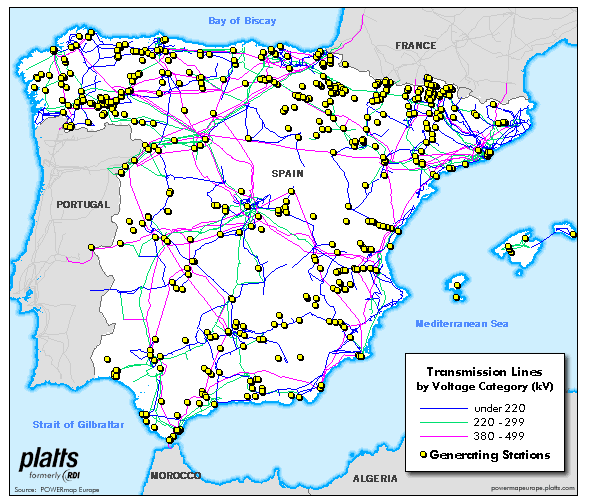
\includegraphics[width=0.8\textwidth]{img/teoria/spain.png}
%   \caption{Red nacional de transmisión energética \cite{spain}}
%   \label{fig:spain}
% \end{figure}





%%%%%%%%%%%%%%%%%%%%%%%%%%%%%%%%%%%%%%%%%%%%%%%%%%%%%%%%%%%%%%%%%%
\subsection{Desafíos futuros de las smart grids}

Las \gls{sg}s, a pesar del progreso tecnológico que han proporcionado en el ámbito de la gestión energética en la última década, no están exentas de desafíos importantes que deben de abordarse para seguir potenciando su crecimiento a futuro. La segunda generación de \gls{sg}s viene dada por la necesidad de implementar las siguientes mejoras: \cite{smartgrid_overview} \cite{ioe}

\begin{itemize}
  \item Inteligencia mejorada: Será preciso poner el foco en el desarrollo de nuevas infraestructuras avanzadas de medición inteligente para afrontar cada vez una mayor demanda y globalizar el mercado energético.
  \item Fortalecimiento de la red: Se debe garantizar una suficiente capacidad de transmisión para favorecer la transmisión de larga distancia y el empleo de fuentes energéticas aisladas, como pueden ser los parques eólicos en el mar.
  \item Adaptación de la red al empleo de vehículos eléctricos: Se requiere preparar la arquitectura de las \gls{sg}s para el creciente uso de vehículos eléctricos que se espera en la próxima década.
  \item Gestión de la generación intermitente y del almacenamiento: Es importante potenciar el empleo de los recursos de generación a pequeña escala, sobre todo en el caso de los entornos residenciales, para conseguir cada vez una mayor descentralización de la red. De la misma manera, se deben abordar las limitaciones actuales que presentan los sistemas de almacenamiento energético para permitir una mayor acumulación de recursos provenientes de fuentes de generación intermitente, como es la solar y la eólica. Esto es imprescindible para garantizar la disponibilidad energética y poder afrontar los posibles picos de demanda que se produzcan a lo largo del tiempo.
  \item Regulación favorable e incentivos económicos: Se puede potenciar la transformación de las redes energéticas mediante el establecimiento de políticas regulatorias que fomenten la inversión \cite{inversion} en \gls{sg}s y mediante colaboraciones entre el sector público y el privado. De la misma forma, implementar estructuras de tarifas de precios dinámicos motivará a un número mayor de usuarios finales a adoptar tecnologías inteligentes para obtener beneficios económicos. 
\end{itemize}


